\documentclass[../eatbrain.tex]{subfile}

\subsection{Struttura}
Grazie alla tipologia di contenuto presente nel sito la struttura generale di quest'ultimo risulta semplice e abbastanza lineare:  ogni sezione infatti presenta al massimo due livelli di profondità, rendendo disponibile l'informazione ricercata in al massimo due click (avendo un'idea precisa di ciò che si vuole trovare). \\
Questa caratteristica è molto utile: l'utente spesso dopo 3 click tende a interrompere la ricerca, provando frustrazione e diminuendo la probabilità di tornare a vistiare il sito.\\
La struttura delle singole pagine è invece uguale per tutte: esclusa la home page che fa una panoramica di tutte le sezioni e necessita di un two columns layout\footnote{http://www.webstyleguide.com/wsg3/6-page-structure/4-page-templates.html} (lasciando il contenuto più corposo nella colonna di sinistra, migliorandone la visibilità), le pagine interne sono disposte ad una colonna sola, rendendo di facile individuazione il contenuto cercato. \\
Le pagine interne di primo livello (quelle collegate direttamente al menù), dovendo esporre un elenco di dati, presentano uno schema a griglia (immagine + titolo) che risulta più efficace di una semplice lista. \\
Un altro punto a favore lo si trova nel layout generico: tutte le pagine infatti hanno uno schema fisso: \\\\
\begin{figure}[h]
	\centering
	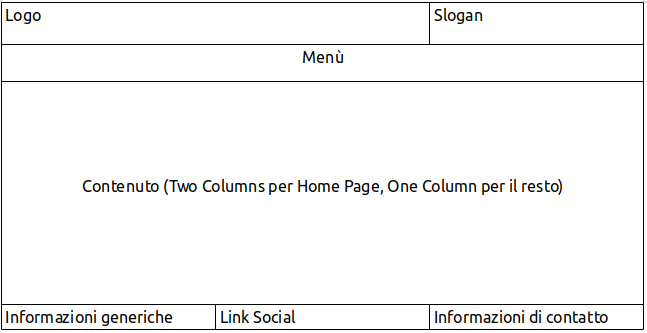
\includegraphics[width=12cm,height=6cm]{immagini/struttura}
	\caption{Struttura generica di tutte le pagine}
	\label{struttura-default}
\end{figure}\\\\
Facilitando l'orientamento all'interno del sito dopo poche interazioni.

\subsection{Navigazione}
No ricerca ma facile orientarsi tramite il menu
No breadcrumb ma evita lost in navigation grazie a struttura semplice
Unica semi pecca grosso scroll per cercare artisti/releases (ricerca browser = sforzo computazionale/ignoranza)
Back button sempre possibile
\subsection{Ricerca}
No ricerca problema nelle pagine a livello più basso (può essere gesitita con ricerca browser ma può richiedere troppo sforzo da parte dell'utente e ignoranza non aiuta)
\subsection{Contenuti Multimediali}
Mannaggia allo slideshow
Caricamento immagine di menu può essere male per connessioni lente
Integrazione soundcloud ottima ma no-javascript no avvisi
Immagine di background non invasiva anzi integrata ottimamente
Immagine header no copy e paste slogan
Immagini release possono aiutare ad orientarsi (lasciano un ricordo di ciò che ho visto)
\subsection{Rispetto Delle Convenzioni}
\subsubsection{Convenzioni Esterne}
No bloated design
No visited link
\subsubsection{Convezioni Interne}
A volta il link è sull'immagine (artisti, macrosezioni) a volte sul testo (releases/podcasts).
\subsection{Gestione degli Errori}
Lost in navigation gestita bene
404 OK,
500 male (/podcasts/)
\subsection{Pubblicità}
Non essendo il sito web la fonte di introito per l'azienda, nessuna pagina presenta pubblicità, rendendo sicuramente più piacevole l'esperienza dell'utente.